\documentclass[journal,twocolumn]{IEEEtran}

%
% Packages:
%
\usepackage{amsmath,amssymb,amsfonts} % For mathematical symbols and environments
\usepackage{algorithmic} % For algorithms (if any, or can be removed)
\usepackage{graphicx} % For including figures (placeholders will be used)
\usepackage{textcomp} % For additional text symbols
\usepackage{xcolor} % For colors (if needed, or can be removed)
\usepackage{cite} % For bibliography management
\usepackage{balance} % To balance columns on the last page
\usepackage{hyperref} % For clickable links, optional

%
% Correct bad hyphenation here
%
\hyphenation{op-tical net-works semi-conduc-tor}


\begin{document}
%
% Paper title
% Titles are generally capitalized except for words such as a, an, and, as,
% at, but, by, for, in, nor, of, on, or, the, to and up, which are usually
% not capitalized unless they are the first or last word of the title.
% Linebreaks \\ can be used within to get better formatting as desired.
% Do not put math or special symbols in the title.
\title{Reinforcement Learning for Channel Estimation in Communications: A Comprehensive Review}
%
%
% author names and IEEE memberships
% note positions of commas and nonbreaking spaces ( ~ ) LaTeX will not break
% a structure at a ~ so this keeps an author's name from being broken across
% two lines.
% use \thanks{} to gain access to the first footnote area
% a separate \thanks must be used for each paragraph of footnote material
\author{SHICHENG CHU, (Student, SZU)% <-this % stops a space
% \thanks{M. Shell was with the Department
% of Electrical and Computer Engineering, Georgia Institute of Technology, Atlanta,
% GA, 30332 USA e-mail: (see http://www.michaelshell.org/contact.html).}% <-this % stops a space
% \thanks{J. Doe and J. Doe are with Anonymous University.}% <-this % stops a space
% \thanks{Manuscript received April 19, 2005; revised August 26, 2015.}
}

% note the % following the last \IEEEmembership and also \thanks -
% these prevent an unwanted space from occurring between the last author name
% and the end of the author line. i.e., if you had this:
%
% \author{....lastname \thanks{...} \thanks{...} }
%                     ^------------^------------^----Do not want these spaces!
%
% a space would be appended to the last name and could cause every name on that
% line to be shifted left slightly. This is one of those "LaTeX things". For
% instance, "\textbf{A} \textbf{B}" will typeset as "A B" not "AB". To get
% "AB" then you have to do: "\textbf{A}\textbf{B}"
% \thanks is no different in this regard, so shield the last } of each \thanks
% that ends a line with a % and do not let a space in before the next \thanks.
% Spaces after \IEEEmembership other than the last one are OK (and needed) as
% you are supposed to have spaces between the names. For what it is worth,
% this is a minor point as most people would not notice if the said evil space
% somehow managed to creep in.



% The paper headers
% \markboth{Journal of Selected Topics in Signal Processing,~Vol.~XX, No.~Y, Month~2025}%
% {Shell \MakeLowercase{\textit{et al.}}: A Sample Article Using IEEEtran.cls for IEEE Journals}
% The only time the second header will appear is for the odd numbered pages
% after the title page when using the twoside option.
%
% *** Note that you probably will NOT want to include the author's ***
% *** name in the headers of peer review papers.                   ***
% You can use \ifCLASSOPTIONpeerreview for conditional compilation here if
% you desire.




% If you want to put a publisher's ID mark on the page you can do it like
% this:
%\IEEEpubid{0000--0000/00\$00.00~\copyright~2025 IEEE}
% Remember, if you use this you must call \IEEEpubidadjcol in the second
% column for its text to clear the IEEEpubid mark.



% use for special paper notices
%\IEEEspecialpapernotice{(Invited Paper)}




% make the title area
\maketitle

% As a general rule, do not put math, special symbols or citations
% in the abstract or keywords.
\begin{abstract}
Accurate channel state information (CSI) plays a pivotal role in modern wireless systems [1]. However, the escalating complexity and inherent dynamics of these systems present formidable challenges to conventional estimation techniques. Reinforcement Learning (RL) emerges as a compelling paradigm, offering the ability to learn optimal strategies through direct interaction with the environment, thereby circumventing the need for explicit mathematical models. This paper provides a comprehensive survey of RL applications in channel estimation, with a particular focus on prominent algorithms such as Q-learning, Deep Q-Networks (DQN), Deep Deterministic Policy Gradient (DDPG), and Proximal Policy Optimization (PPO). Key achievements are underscored, particularly in optimizing Intelligent Reflecting Surface (IRS) configurations, estimating time-varying channels, enhancing Multiple-Input Multiple-Output (MIMO) systems, and enabling end-to-end communication frameworks. RL-driven methods have shown considerable advantages over conventional approaches, notably in reducing estimation error and enhancing system-level metrics. Despite these advancements, challenges such as computational overhead and generalization capabilities persist. Accordingly, this review also delves into promising future research avenues, including meta-RL, the development of lightweight algorithms, and holistic optimization strategies. Ultimately, this review seeks to foster a deeper understanding of RL's potential in tackling the intricate channel estimation problems anticipated in next-generation wireless networks.
\end{abstract}

% Note that keywords are not normally used for peerreview papers.
\begin{IEEEkeywords}
Reinforcement Learning, Channel Estimation, Wireless Communications, Deep Learning, Machine Learning, 5G, 6G, Intelligent Reflecting Surface (IRS), MIMO, Dynamic Channels, End-to-End Learning.
\end{IEEEkeywords}


% For peer review papers, you can put extra information on the cover
% page as needed:
% \ifCLASSOPTIONpeerreview
% \begin{center} \bfseries EDICS Category: 3-BBND \end{center}
% \fi
%
% For peerreview papers, this IEEEtran command inserts a page break and
% creates the second title. It will be ignored for other modes.
\IEEEpeerreviewmaketitle



\section{Introduction}
% IEEEtranNWS [showrules] V1.8b enabled.

\IEEEPARstart{T}{he} relentless evolution of wireless communication systems towards 5G/6G, characterized by innovations such as massive Multiple-Input Multiple-Output (MIMO), the exploitation of millimeter-Wave (mmWave)/Terahertz (THz) frequencies, and the advent of Intelligent Reflecting Surfaces (IRS), has amplified the dependence on precise Channel State Information (CSI) [1]. Furthermore, the integration of Mobile Edge Computing (MEC) technologies [27] adds another layer of complexity to modern wireless networks, necessitating sophisticated channel estimation approaches. In these intricate scenarios, traditional estimation methods encounter substantial hurdles. For instance, massive MIMO systems give rise to high-dimensional channel matrices, while vehicular and other high-mobility applications induce rapidly varying channels that defy quasi-static assumptions. Furthermore, the inherent sensitivity of mmWave communications and the complex cascaded channels introduced by IRS complicate accurate modeling. A common recourse, increasing pilot overhead for improved estimation accuracy, invariably compromises spectral efficiency. Against this backdrop, Reinforcement Learning (RL) has emerged as a powerful alternative, learning optimal policies through environmental interaction without necessitating explicit models or labeled data, rendering it particularly adept at navigating the complexities of modern wireless channels. RL agents learn to adaptively select pilots, optimize IRS configurations, denoise estimates, track variations, and even optimize end-to-end communication parameters. Deep Reinforcement Learning (DRL), which synergistically combines RL with the representational power of deep neural networks, effectively handles the high-dimensional state and action spaces typical in contemporary wireless communications. To this end, this review delineates the landscape of RL applications in channel estimation. We delve into the core methodologies, survey significant research achievements across a spectrum of communication scenarios, benchmark performance enhancements relative to conventional techniques, critically examine inherent challenges, and outline promising trajectories for future research.

\section{Reinforcement Learning Methodologies for Channel Estimation}

Reinforcement Learning provides a robust framework wherein an agent learns to make optimal decisions by interacting with an environment. In the context of channel estimation, RL algorithms endeavor to learn policies that improve estimation accuracy or enhance overall system performance, often without relying on explicit channel models [6]. Several distinct RL methodologies have been brought to bear on channel estimation problems, each possessing unique strengths suited to specific scenarios.

Value-based methods focus on learning a value function that estimates the expected return for taking a particular action in a given state. Q-learning, a foundational value-based approach, aims to learn the optimal action-value function, denoted as $Q^*(s, a)$, which represents the maximum expected future reward achievable by taking action $a$ in state $s$ and subsequently following the optimal policy. For discrete state and action spaces, Q-values are typically stored in a tabular format and updated iteratively using the Bellman equation: $Q(s_t, a_t) \leftarrow Q(s_t, a_t) + \alpha [r_{t+1} + \gamma \max_{a'} Q(s_{t+1}, a') - Q(s_t, a_t)]$, where $\alpha$ is the learning rate and $\gamma$ is the discount factor. The discrete nature of action selection inherent in certain channel estimation sub-problems, such as choosing optimal precoding matrices from a finite set or deciding on specific denoising levels, makes Q-learning a natural fit. Indeed, its utility has been demonstrated in applications like channel prediction for Non-Orthogonal Multiple Access (NOMA) systems and iterative denoising processes in MIMO-Orthogonal Frequency Division Multiplexing (OFDM) architectures, where the agent refines its policy for action selection based on evolving channel state representations.

For problems characterized by large or continuous state spaces, prevalent in modern wireless systems, traditional Q-tables become impractical due to the "curse of dimensionality." Deep Q-Networks (DQN) address this limitation by employing deep neural networks to approximate the Q-function, $Q(s, a; \theta)$, where $\theta$ represents the network weights. DQNs integrate techniques such as experience replay (storing and randomly sampling past transitions) and target networks (using a separate, periodically updated network) to bolster stability and performance. The capacity of DQN to handle vast state spaces has proven beneficial in scenarios like Internet of Things (IoT) backscatter communications [9], where channel conditions can be highly variable and numerous, and in optimizing parameters crucial for adaptive channel equalization.

Policy gradient methods adopt a different strategy by directly learning the policy function $\pi(a|s; \theta)$, which maps states to actions. The policy parameters $\theta$ are updated via gradient ascent on an objective function that quantifies the expected cumulative reward. Actor-critic methods amalgamate value-based and policy-based approaches, typically comprising an Actor that learns and implements the policy $\pi(a|s; \theta)$ and a Critic that learns a value function to evaluate the actor's actions, thereby guiding policy updates.

Deep Deterministic Policy Gradient (DDPG) is an actor-critic, model-free algorithm specifically designed for continuous action spaces, which are frequently encountered in wireless communication problems. DDPG learns a deterministic policy (Actor) and an action-value function (Critic), leveraging experience replay and target networks akin to DQN. It has been successfully applied to optimizing IRS configurations, where the action space (phase shifts) is continuous [7], and in end-to-end communication systems, where the transmitter learns to encode signals without explicit channel knowledge [5].

Proximal Policy Optimization (PPO) aims for more stable and reliable policy updates compared to vanilla policy gradient methods by utilizing a clipped surrogate objective function that constrains policy changes at each iteration. Although PPO might not always be tasked with the direct inference of channel coefficients, its strength in policy optimization under constraints makes it valuable for adjusting system parameters that are intrinsically linked to, or reliant upon, the underlying channel state. Illustrative applications include resource allocation in Reconfigurable Intelligent Surface (RIS)-assisted Mobile Edge Computing (MEC) systems [7], where decisions are conditioned on channel quality, and the design of efficient channel sampling patterns in Integrated Sensing and Communications (ISAC) frameworks [19].

Twin Delayed Deep Deterministic Policy Gradient (TD3) extends DDPG to mitigate overestimation bias and enhance stability through mechanisms like clipped double Q-learning, delayed policy updates, and target policy smoothing. TD3 has found application in RIS-assisted networks for optimizing phase-shift matrices [8] and for signal detection in RIS-assisted ambient backscatter communication.

The selection of an appropriate RL algorithm for channel estimation depends on several factors: the nature of the state and action spaces (discrete vs. continuous), the complexity of the problem, computational constraints, and the desired trade-off between sample efficiency and performance. Value-based methods like Q-learning and DQN are typically preferred for discrete action spaces, while policy gradient and actor-critic methods like DDPG, PPO, and TD3 are better suited for the continuous action spaces often encountered in wireless channel optimization problems. As wireless systems become increasingly complex, the trend is toward more sophisticated algorithms that can effectively handle high-dimensional, continuous spaces while maintaining sample efficiency and computational feasibility.

\begin{figure}[!t]
\centering
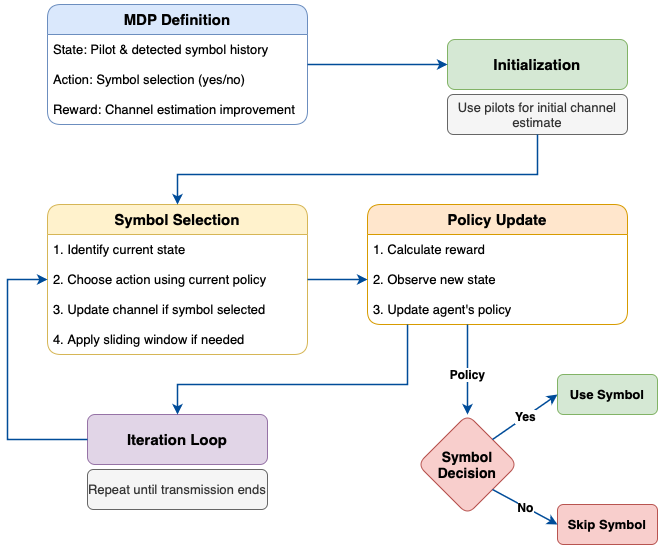
\includegraphics[width=0.9\columnwidth]{fig_symbol_selection_mdp.png}
\caption{A typical MDP framework for RL-based symbol selection in channel estimation}
\label{fig:symbol_selection_mdp}
\end{figure}

\section{Applications and Achievements Across Communication Scenarios}

Reinforcement Learning has demonstrated significant potential across a diverse array of communication scenarios where channel estimation poses unique and often formidable challenges. These applications effectively showcase RL's versatility and its efficacy in adapting to complex and dynamic channel environments.

In Intelligent Reflecting Surface (IRS) deployments, RL algorithms are employed to dynamically optimize the phase shifts of reflecting elements, thereby actively manipulating wireless channels. DRL approaches, including DDPG [7], DQN, PPO, and TD3 [8], empower an agent to observe relevant channel state information and adjust IRS configurations to maximize pertinent metrics such as sum-rate, Signal-to-Interference-plus-Noise Ratio (SINR), coverage, or energy efficiency. Empirical studies and simulations consistently reveal RL's proficiency in adaptively tailoring IRS configurations to dynamic environmental shifts, thereby achieving notable gains in signal quality and overall system performance when benchmarked against traditional optimization heuristics. While the primary focus is often on IRS configuration, this process is intrinsically linked to channel estimation, as the agent learns policies that implicitly account for and adapt to underlying channel characteristics.

\begin{figure}[h!]
\centering
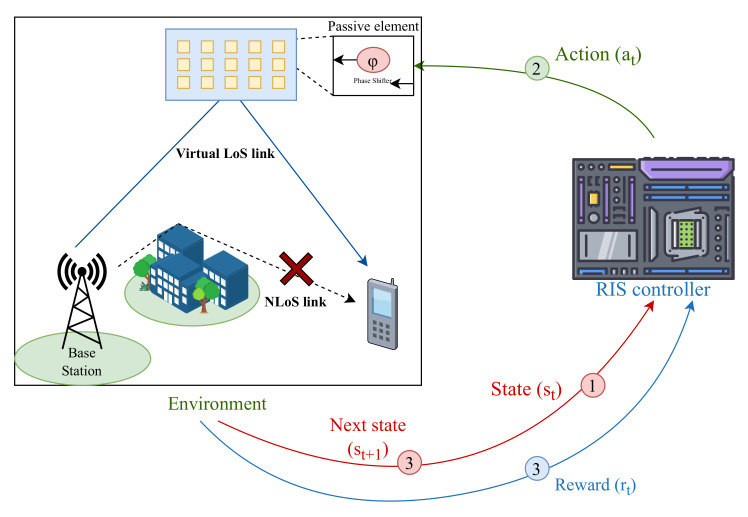
\includegraphics[width=0.8\columnwidth]{Reinforcement learning model.png}
\caption{Reinforcement learning framework for IRS-assisted communication systems}
\label{fig:rl_irs_framework}
\end{figure}

For time-varying and doubly dispersive channels, commonly encountered in high-mobility scenarios such as Vehicle-to-Everything (V2X) communications and high-speed rail, traditional estimation methods predicated on quasi-static channel assumptions tend to perform poorly. RL offers an adaptive framework where agents can, for instance, select optimal detected data symbols to aid in data-aided channel estimation [8, 4]. The Markov Decision Process (MDP) formulation typically involves states representing historical channel information and detected symbols, with rewards structured to reflect estimation accuracy. Estimators augmented by RL have exhibited tangible improvements in Bit Error Rate (BER) and Normalized Mean Squared Error (NMSE), particularly under conditions of pronounced channel variability where conventional techniques often falter.

In MIMO and massive MIMO systems, the high dimensionality of channel matrices presents substantial estimation challenges. Q-learning has been applied to tasks like successive channel denoising in MIMO-OFDM systems [18], where the agent learns to identify and refine unreliable channel estimates based on metrics like channel curvature. Low-complexity RL algorithms have also been developed for selecting detected data symbols to aid channel estimation, achieving a reduction in computational complexity while simultaneously improving BER and NMSE [14]. Beyond the direct inference of channel parameters, RL methodologies are also being harnessed for astute resource allocation in massive MIMO deployments. In such schemes, the agent, by making decisions informed by observed CSI or related quality indicators, implicitly learns to navigate and adapt to the intricacies of the high-dimensional channel milieu [15].

A more radical approach involves end-to-end (E2E) communication systems using DRL to learn the entire communication system without explicit channel models. The DDPG-E2E framework [5, 11] treats the transmitter as an RL agent that learns to encode messages into signals, with the wireless channel as an unknown environment. The transmitter and receiver jointly learn to adapt to channel characteristics through the E2E training process, effectively treating the channel as a "black box." This approach can discover novel communication schemes optimized for specific unknown channels and demonstrates better BLER performance and convergence rates compared to state-of-the-art solutions over complex wireless channels [5].

\begin{figure}[!t]
\centering
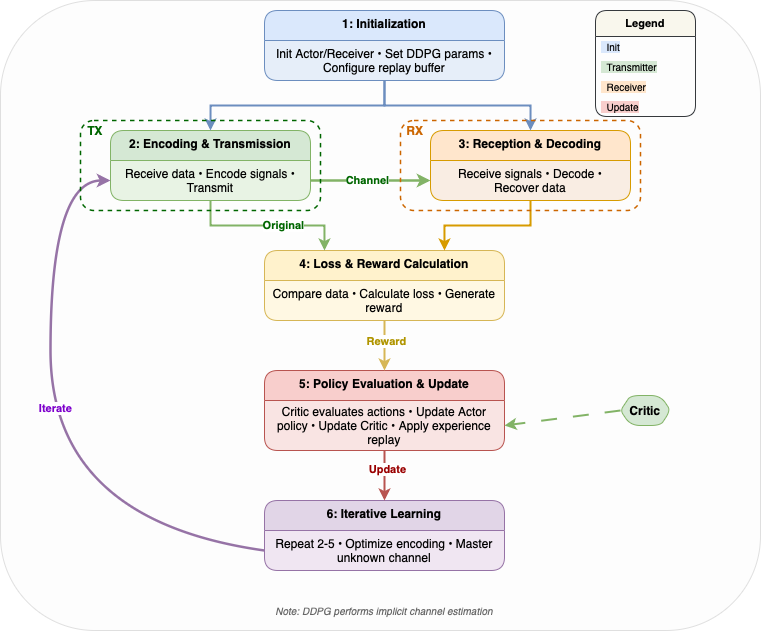
\includegraphics[width=\columnwidth]{fig_ddpg_e2e.png}
\caption{DDPG-E2E learning framework for end-to-end communication systems}
\label{fig:ddpg_e2e}
\end{figure}

RL is also finding applications in emerging wireless scenarios with unique channel challenges. In millimeter-wave (mmWave) communications, RL is used to jointly optimize hybrid beamforming matrices and ADC threshold levels in systems with low-resolution ADCs, maximizing achievable rates by adapting to channel statistics while remaining robust to noisy CSI estimates [20]. For IoT and backscatter communications, DRL (including DQN, DDQN, DDPG, PPO) enhances channel estimation by enabling devices to adapt their transmission parameters and estimation policies based on changing SNR and interference, leading to more accurate estimates and improved system performance [9]. RL also optimizes resource allocation, packet scheduling, and network selection in these low-power scenarios.

V2X communication channels present particularly demanding conditions characterized by high mobility, rapid temporal variations, and inherent non-stationarity. Current RL research in this domain often focuses on resource allocation, spectrum sharing, and adaptive beamforming strategies designed to cope with these dynamic channel conditions [11, 12, 13]. Machine learning approaches for vehicular networks have shown considerable promise in addressing the unique challenges of communication, computation, and security in these environments [23]. DRL is employed, for example, to optimize beamforming and power allocation in Integrated Sensing and Communications (ISAC) for V2X, aiming to reduce reliance on extensive pilot signals by leveraging sensing state information [13]. While not always directly estimating channel coefficients, these systems learn to operate effectively within the challenging V2X propagation environments.

\begin{figure}[!b]
\centering
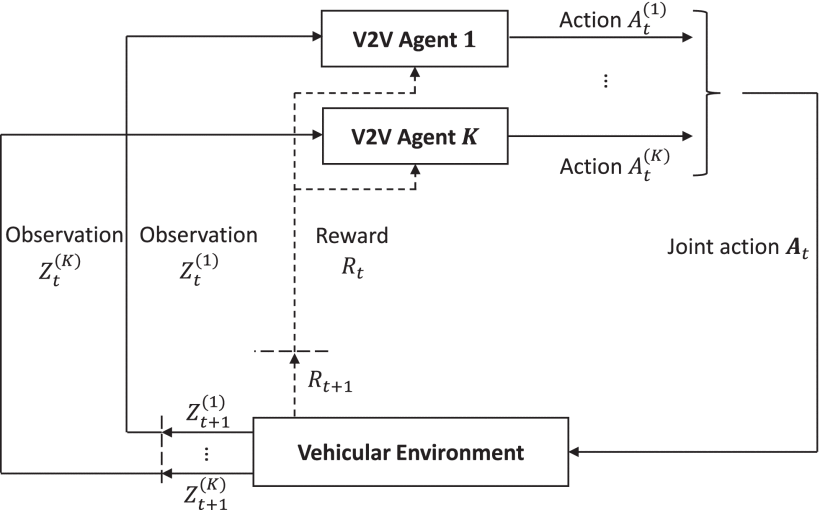
\includegraphics[width=\columnwidth]{fig_marl_v2x_spectrum_sharing.png}
\caption{Multi-agent reinforcement learning framework for V2X spectrum sharing}
\label{fig:marl_v2x}
\end{figure}

Even in the domain of underwater acoustic communications, notorious for long multipath delays, significant Doppler shifts, and severely limited bandwidth, DRL approaches such as Long Short-Term Memory (LSTM)-DQN have been applied to adaptive modulation based on outdated or predicted CSI, reportedly outperforming traditional methods [16]. Some research also explores model-based RL frameworks to recursively estimate channel model parameters and track their dynamics in these challenging underwater environments [16].

Across this diverse spectrum of scenarios, RL provides a flexible and adaptive framework to tackle the intricacies of channel estimation, either through direct inference or by optimizing systems to work efficiently with available or imperfect channel information. The consistent underlying theme is RL's ability to learn effective operational policies in complex, dynamic environments where traditional model-based approaches often struggle, rendering it particularly valuable for the demands of next-generation wireless communications.

\section{Performance Benchmarks and Achievements}

The application of Reinforcement Learning to channel estimation has yielded notable achievements, quantifiable across multiple performance metrics. These benchmarks underscore RL's potential to enhance not only estimation accuracy but also overall system performance, often surpassing traditional approaches.

A primary testament to RL's efficacy in channel estimation is the consistent observation of reduced estimation error. In IRS-assisted systems, for instance, DRL approaches that integrate Convolutional Neural Networks (CNNs) and Gated Recurrent Units (GRUs) with DDPG have achieved markedly smaller channel estimation errors (NMSE) for both direct and cascaded channels when compared to traditional Least Squares (LS) and Linear Minimum Mean Squared Error (LMMSE) methods [7]. Similarly, in MIMO-OFDM systems, Q-learning based successive denoising methods have demonstrated an ability to approach the Mean Squared Error (MSE) performance of ideal LMMSE (which requires perfect channel statistics) and have offered substantial gains (approximately 6 dB) over basic LS estimation [18]. Furthermore, low-complexity RL algorithms designed for MIMO systems have reported significant reductions in NMSE compared to their conventional counterparts [14].

These improvements in estimation accuracy often translate directly into enhanced system-level performance. RL-aided channel estimators for time-varying MIMO systems have demonstrated better BLER than conventional pilot-aided methods [8, 4]. Specifically, low-complexity RL estimators have achieved BER improvements of approximately 0.7-1.2 dB at a BLER of $10^{-1}$ [14]. DDPG-E2E systems have showcased superior BLER performance and faster convergence rates over complex wireless channels when contrasted with other E2E learning solutions [5]. In terms of throughput, Q-learning applied to channel prediction in Multiple-Input Single-Output (MISO)-NOMA systems has been shown to enhance the sum rate compared to standard Minimum Mean Square Error (MMSE) and DL-based LSTM procedures [17]. Concurrently, DRL-optimized IRS configurations have led to higher achievable system rates, particularly after co-optimization with beamforming strategies [7]. RL-based optimization of beamforming and ADC thresholds in mmWave MIMO systems has closely matched the performance of exhaustive search methods and significantly outperformed traditional baselines in terms of achievable rates [20].

Beyond sheer accuracy, RL-based strategies often confer enhanced robustness and adaptability to the estimation process. Agents can learn to adapt to dynamic channel environments where traditional methods may struggle, a capability particularly valuable in time-varying channels [8, 4] and IRS-equipped systems [7]. A distinct advantage of many RL formulations, particularly when contrasted with supervised Deep Learning (DL) techniques, is their capacity to operate effectively even without perfect a priori channel knowledge or extensive pre-labeled datasets. DDPG-E2E systems exemplify this adaptability by jointly training transmitters and receivers over unknown channels [5].

In certain applications, RL can also contribute to reduced overhead and complexity. By learning to select optimal data symbols for estimation or by enabling end-to-end learning paradigms, RL can potentially diminish the reliance on extensive pilot signaling. Research into low-complexity RL algorithms actively aims to make these sophisticated solutions practical for real-world deployment by reducing the computational demands compared to initial, more complex DRL proposals [14]. For example, techniques such as using sub-blocks and backup samples have been shown to significantly reduce computational complexity and latency without a concomitant loss in performance in some RL-aided channel estimators [4].

While quantitative comparisons invariably depend on the specific scenario, chosen baseline methods, and evaluation metrics, the overarching trend indicates that RL holds significant potential for pushing the boundaries of channel estimation performance. This is particularly true for the complex and dynamic environments characteristic of next-generation wireless systems. This inherent capability to learn and adapt through environmental interaction furnishes a potent alternative to conventional model-based approaches, which often see their performance degrade when underlying model assumptions are inevitably violated in real-world scenarios.

\section{Challenges and Practical Considerations}

Despite the promising results and demonstrable potential, the practical application of Reinforcement Learning in channel estimation is confronted by several challenges that must be systematically addressed to realize its full potential in real-world wireless systems.

Computational complexity and latency represent significant hurdles. DRL algorithms, especially those incorporating deep neural networks, can be computationally intensive to train, typically requiring substantial datasets and considerable processing power [14, 4, 8]. The deployment of such algorithms in edge computing environments [24, 25] further complicates the computational considerations, as resource constraints at the edge necessitate careful optimization of algorithm complexity. This computational burden is particularly acute for resource-constrained end-user devices or edge nodes, and can also hinder responsiveness in scenarios with rapidly decorrelating channel conditions where timely estimates are paramount. Even after the training phase, the inference time of complex DRL agents might exceed the stringent latency requirements imposed by real-time channel estimation tasks. While traditional Q-learning avoids neural network complexity, it faces the "curse of dimensionality," where the size of the Q-table grows exponentially with the state and action spaces [17], limiting its applicability in complex scenarios.

Sample efficiency and convergence speed also pose considerable challenges. RL agents typically necessitate a multitude of interactions with the environment to learn effective policies. Within the wireless communications context, this often translates into a need for prolonged training phases or a greater reliance on pilot transmissions for sufficient environmental interaction, both of which can impinge upon overall spectral efficiency. Convergence to optimal or near-optimal policies can be slow, particularly in intricate environments characterized by sparse rewards or extended episode lengths.

Adaptation to highly dynamic and non-stationary environments presents another layer of difficulty. While RL is inherently designed for dynamic scenarios, extremely fast-changing channel conditions can still prove problematic. Policies learned under one specific set of channel statistics might exhibit suboptimal performance if these conditions change drastically and rapidly [8, 4]. Potential delays in the decision-making loop of an RL agent can adversely affect real-time performance, especially in fast-fading channels [7].

The design of efficacious reward functions is itself a non-trivial endeavor. Crafting appropriate reward functions that accurately encapsulate channel estimation objectives (e.g., minimizing NMSE, maximizing system throughput) and effectively guide the agent's learning process requires careful consideration and domain expertise. Sparse or significantly delayed rewards—for example, where the ultimate impact of a channel estimation decision on metrics like BER only crystallizes after numerous subsequent communication steps—can substantially complicate and prolong the learning process.

Generalization and robustness concerns also warrant attention. Policies meticulously trained in specific simulation environments may not generalize effectively to diverse real-world deployment scenarios with different channel characteristics or interference patterns. RL agents can exhibit sensitivity to hyperparameter settings, often requiring extensive tuning for optimal performance. Some studies have observed performance saturation at high Signal-to-Noise Ratios (SNRs), where the learning models struggle to achieve estimation errors that are infinitesimally close to zero [7].

Additional challenges include the judicious definition of appropriate state and action spaces, striking the right balance between exploration (discovering new strategies) and exploitation (leveraging known good strategies), and addressing application-specific issues. For instance, in IRS-assisted systems, the continuous acquisition of accurate CSI to facilitate effective optimization in dynamic environments remains a persistent challenge [8]. Data-aided estimation techniques inherently risk error propagation if symbols used for estimation are detected incorrectly [8, 14]. End-to-end learning systems, while promising in their holistic approach, often present difficulties in terms of understanding the learned policies and ensuring their interpretability [11].

Furthermore, akin to other machine learning paradigms, DRL-based channel estimation systems are not immune to security vulnerabilities. They may be susceptible to carefully crafted adversarial attacks aimed at degrading estimation fidelity or even compromising the integrity of the communication link [10]. The security and privacy challenges in mobile edge computing [21, 22] become particularly relevant when RL-based channel estimation is deployed in MEC environments, where additional vulnerabilities may arise from the distributed nature of computation. Blockchain-based security mechanisms [30] present potential solutions for securing AI-driven communication systems.

Addressing these multifaceted limitations through continued algorithmic innovations, the development of more efficient learning paradigms, and careful system-level design will be essential for the widespread and successful adoption of RL in practical channel estimation applications.

\section{Future Research Directions}

The application of Reinforcement Learning to channel estimation continues to be a vibrant area of research, with several promising directions emerging to address current limitations and extend existing capabilities. These innovations are primarily focused on enhancing the intelligence, efficiency, robustness, and practical deployability of RL-based solutions.

Advanced learning paradigms represent a significant frontier. Meta-Reinforcement Learning (Meta-RL) endeavors to train agents that can quickly adapt to new and unseen channel environments with minimal additional training data. By acquiring experience across a diverse ensemble of channel estimation tasks, Meta-RL aims to distill 'meta-knowledge,' enabling the formulation of adaptable meta-policies. These policies can then be rapidly specialized to novel, previously unseen channel conditions with remarkably few additional learning iterations. Model-Agnostic Meta-Learning (MAML) and its variants have shown promise for applications such as time-varying OFDM channel estimation [3, 2], enabling networks to adapt to new tasks with a limited number of training samples. Transfer learning operates on a similar principle, leveraging knowledge acquired in source environments to improve learning performance and speed in target scenarios. Deep Transfer Learning (DTL) has been applied to tasks like downlink channel prediction in Frequency Division Duplex (FDD) massive MIMO systems [2] and to accelerate the convergence of Heterogeneous Federated Learning for channel estimation [3]. As privacy concerns become increasingly prominent, Federated Reinforcement Learning offers a framework where multiple agents can collaboratively train global models without sharing their raw channel data. This distributed approach has been explored for RIS-assisted cell-free MIMO systems [3], offering potential benefits in terms of enhanced privacy, reduced communication overhead, and improved scalability.

Developing lightweight and computationally efficient DRL algorithms is crucial for practical deployment, especially on resource-constrained devices such as IoT sensors and mobile terminals. Research in this area focuses on techniques like network pruning and quantization to reduce the size and computational footprint of deep neural networks, knowledge distillation to train smaller "student" networks that emulate the performance of larger "teacher" networks, the design of more efficient exploration strategies to reduce sample requirements, and the development of inherently low-complexity RL algorithms [14]. Mobile edge computing architectures [26, 28] offer promising platforms for deploying these lightweight algorithms, providing a balance between computational capability and proximity to end devices. The overarching goal of these research endeavors is to render DRL-based channel estimation practically viable for on-device learning, particularly within the constraints of mobile and IoT hardware, and to ensure real-time operational capability across an expanding gamut of wireless applications.

Robust Reinforcement Learning constitutes another important avenue of investigation. Wireless channels can be inherently adversarial, subject to unpredictable interference, intentional jamming, or sudden and drastic changes in propagation conditions. Designing RL agents that can maintain effective performance despite such uncertainties, disturbances, and potential malicious attacks involves drawing upon techniques from robust optimization and game theory. The integration of RL with IRS, for instance, can inherently improve robustness by providing a mechanism to adaptively reconfigure the propagation environment itself [7], while secure channel estimation that explicitly considers and mitigates adversarial attacks remains an active and critical research area [10].

As DRL models become increasingly complex, often functioning as "black boxes," the integration of Explainable AI (XAI) techniques becomes essential. Understanding the rationale behind an agent's decisions is crucial for debugging, fostering trust, and facilitating certification for deployment in critical systems. Developing XAI approaches tailored for DRL in channel estimation contexts can provide valuable insights into learned policies and decision-making processes. This not only increases trustworthiness but can also facilitate a deeper understanding of the underlying channel physics that the agents implicitly learn.

A particularly ambitious yet promising frontier involves holistic optimization. Channel estimation is not an isolated task; its quality directly impacts a multitude of higher-layer operations, including resource allocation, beamforming, scheduling, and ultimately, application-level Quality of Service (QoS). Here, RL could serve as the linchpin for jointly optimizing channel estimation in concert with other interdependent communication tasks, such as resource allocation, beamforming, and scheduling. Enterprise-level MEC deployments [29] provide ideal testbeds for such holistic optimization approaches, where multiple communication and computation tasks can be jointly optimized. Such an integrated approach has the potential to unlock synergistic gains and achieve superior end-to-end system performance that might be unattainable through piecemeal optimization. Examples already emerging include end-to-end communication systems where DDPG jointly optimizes transmitter and receiver functionalities [5], RL agents that dynamically adapt their estimation strategies based on prevailing network load or QoS requirements, and joint optimization of IRS phase shifts in conjunction with resource allocation policies.

The pursuit of these innovative research directions promises to further solidify RL's role as a key enabler for intelligent and adaptive channel estimation in future wireless communication systems. As research continues to refine algorithms, address current limitations, and explore new synergistic combinations with other AI techniques, we can anticipate significant advancements in the effectiveness, practicality, and trustworthiness of RL-based channel estimation approaches for the next generation of wireless networks.

\section{Conclusion}

The relentless march of wireless communications towards unprecedented complexity, dynamism, and diverse service demands underscores the imperative for innovative paradigms to address fundamental challenges such as channel estimation. Reinforcement Learning, particularly when augmented by the representational power of Deep Learning, has emerged as a transformative framework, seemingly ideally suited to navigate the intricacies of modern wireless channels. Its inherent ability to learn from interaction, adapt dynamically without explicit models, and optimize for long-term strategic goals directly addresses many of the limitations faced by conventional estimation techniques in the context of next-generation networks.

Throughout this review, we have navigated the burgeoning landscape of RL applications within channel estimation. We have seen its utility in actively shaping wireless environments through intelligent surface control, enhancing estimation accuracy in highly time-varying channels, enabling novel end-to-end communication paradigms that bypass traditional layered approaches, and optimizing critical system parameters in challenging domains such as mmWave, IoT, and V2X communications. The consistent reports of performance improvements—manifested in reduced estimation error, lower bit error rates, enhanced throughput, and greater adaptability—collectively demonstrate RL's profound potential to push beyond the performance envelopes of established traditional approaches.

Nevertheless, the trajectory towards widespread, practical deployment is not without its hurdles, necessitating concerted efforts to address the aforementioned challenges. Computational demands, limitations in sample efficiency, ensuring robust adaptation to highly non-stationary environments, the intricacies of reward function design, and concerns regarding generalization all represent active and critical areas of ongoing research. The "black-box" nature of many complex DRL models also calls for greater attention to developing methods for explainability and interpretability.

Future directions in this vibrant field are rich with potential. Advanced learning paradigms like meta-RL and transfer learning hold the promise of accelerating adaptation and significantly reducing data requirements. The development of lightweight algorithms will be instrumental in enabling practical deployment on resource-constrained devices. The creation of robust agents will ensure sustained performance even in the face of adversarial conditions or unexpected environmental shifts. Holistic optimization frameworks, which integrate channel estimation with broader system objectives, have the potential to yield globally optimized performance, unlocking new efficiencies.

As wireless systems inexorably advance in sophistication and functional capability, the core tenets of RL—adaptive learning, data-driven optimization, and goal-oriented behavior—appear increasingly, and perhaps fundamentally, aligned with the pressing requirements of next-generation networks. Although challenges undoubtedly persist, the overarching trajectory suggests that RL-based approaches are poised to assume an increasingly pivotal role. They promise to imbue wireless communication systems with greater intelligence, efficiency, and resilience, thereby unlocking novel capabilities and potentially redefining the performance frontiers not only in channel estimation but across the broader communications domain.

\begin{thebibliography}{30} % <-- 请根据您的总文献数量修改此处的数字 (e.g., {25} or {99})

\bibitem{1}
V. W. Wong, R. Schober, D. W. K. Ng, and L. C. Wang, \emph{Key Technologies for 5G Wireless Systems}. Cambridge University Press, 2017.

\bibitem{2}
P. Tarafder, C. Chun, A. Ullah, Y. Kim, and W. Choi, "Channel Estimation in 5G-and-Beyond Wireless Communication: A Comprehensive Survey," \emph{Electronics}, vol. 14, no. 4, p. 750, 2025.

\bibitem{3}
X. Liu, S. Zhao, Y. Liang, and S. Karim, "Research on channel estimation based on joint perception and deep enhancement learning in complex communication scenarios," \emph{PeerJ Computer Science}, vol. 11, p. e2852, 2025.

\bibitem{4}
T.-K. Kim and M. Min, "Reinforcement Learning-Aided Channel Estimator in Time-Varying MIMO Systems," \emph{Sensors}, vol. 23, no. 12, p. 5689, 2023.

\bibitem{5}
B. Zhang, N. Van Huynh, D. T. Hoang, D. N. Nguyen, and Q.-V. Pham, "DDPG-E2E: A Novel Policy Gradient Approach for End-to-End Communication Systems," \emph{IEEE Transactions on Cognitive Communications and Networking}, 2024.

\bibitem{6}
J. Wang, C. Jiang, H. Zhang, Y. Ren, K.-C. Chen, and L. Hanzo, "Thirty years of machine learning: The road to Pareto-optimal wireless networks," \emph{IEEE Communications Surveys \& Tutorials}, vol. 22, no. 3, pp. 1472--1514, 2020.

\bibitem{7}
P. S. Aung, S. M. Kang, and C. S. Hong, "Proximal Policy Optimization for Energy-Efficient MEC Systems with STAR-RIS Assistance," in \emph{2024 International Conference on Information Networking (ICOIN)}, pp. 239--244, 2024.

\bibitem{8}
A. A. Puspitasari and B. M. Lee, "A survey on reinforcement learning for reconfigurable intelligent surfaces in wireless communications," \emph{Sensors}, vol. 23, no. 5, p. 2554, 2023.

\bibitem{9}
W. U. Khan, E. Lagunas, Z. Ali, A. Mahmood, C. K. Sheemar, M. Ahmed, K. Dev, S. Chatzinotas, and B. Ottersten, "Deep Reinforcement Learning for Backscatter Communications: Augmenting Intelligence in Future Internet of Things," \emph{IEEE Internet of Things Magazine}, vol. 7, no. 5, pp. 72--78, 2024.

\bibitem{10}
K. Ullah, S. Jian, M. N. U. Hassan, S. Khan, M. Babar, A. Ahmad, and S. Ahmad, "Secure Channel Estimation Using Norm Estimation Model for 5G Next Generation Wireless Networks," \emph{Computers, Materials \& Continua}, vol. 82, no. 1, 2025.

\bibitem{11}
R. Dinesh Deshpande, F. A. Khan, and Q. Zeeshan Ahmed, "Spectrum Sharing using Deep Reinforcement Learning in Vehicular Networks," \emph{arXiv e-prints}, pp. arXiv--2410, 2024.

\bibitem{12}
L. Liang, H. Ye, and G. Y. Li, "Spectrum sharing in vehicular networks based on multi-agent reinforcement learning," \emph{IEEE Journal on Selected Areas in Communications}, vol. 37, no. 10, pp. 2282--2292, 2019.

\bibitem{13}
C. Shang, J. Yu, and D. T. Hoang, "Energy-Efficient and Intelligent ISAC in V2X Networks with Spiking Neural Networks-Driven DRL," \emph{arXiv preprint arXiv:2501.01038}, 2025.

\bibitem{14}
T.-K. Kim and M. Min, "A low-complexity algorithm for a reinforcement learning-based channel estimator for MIMO systems," \emph{Sensors}, vol. 22, no. 12, p. 4379, 2022.

\bibitem{15}
T. Chen, B. Ji, Y. Shi, T. Ding, B. Fang, S. Yi, and X. Tu, "Neural network compression via sparse optimization," \emph{arXiv preprint arXiv:2011.04868}, 2020.

\bibitem{16}
Y. Zhang, J. Zhu, H. Wang, X. Shen, B. Wang, and Y. Dong, "Deep reinforcement learning-based adaptive modulation for underwater acoustic communication with outdated channel state information," \emph{Remote Sensing}, vol. 14, no. 16, p. 3947, 2022.

\bibitem{17}
M. Gaballa, M. Abbod, and A. Aldallal, "A study on the impact of integrating reinforcement learning for channel prediction and power allocation scheme in MISO-NOMA system," \emph{Sensors}, vol. 23, no. 3, p. 1383, 2023.

\bibitem{18}
M. S. Oh, S. Hosseinalipour, T. Kim, C. G. Brinton, and D. J. Love, "Channel estimation via successive denoising in MIMO OFDM systems: A reinforcement learning approach," in \emph{ICC 2021-IEEE International Conference on Communications}, 2021, pp. 1--6.

\bibitem{19}
F. Mason and J. Pegoraro, "Using Deep Reinforcement Learning to Enhance Channel Sampling Patterns in Integrated Sensing and Communication," \emph{IEEE Wireless Communications Letters}, 2024.

\bibitem{20}
M. T. Alonso, D. Luo, and F. Shirani, "Deep Reinforcement Learning for MIMO Communication with Low-Resolution ADCs," \emph{arXiv preprint arXiv:2504.18957}, 2025.

\bibitem{21}
A. A. C. Manogaran, V. Varatharajan, and C. H. Hsu, "A Survey of Security and Privacy in Mobile Edge Computing," \emph{ACM Computing Surveys}, vol. 52, no. 6, article 122, pp. 1--36, Dec. 2019.

\bibitem{22}
C. A. Kerr, "A Survey on Security and Privacy Issues in Mobile Edge Computing," \emph{Journal of Network and Computer Applications}, vol. 147, p. 102434, Dec. 2019.

\bibitem{23}
Y. Sun, J. Liu, Y. Wang, X. Zhang, and N. Kato, "When Machine Learning Meets Vehicular Networks: A Survey on Communication, Computation, and Security," \emph{IEEE Communications Surveys \& Tutorials}, vol. 22, no. 4, pp. 2298--2333, Fourthquarter 2020.

\bibitem{24}
W. Z. Khan, E. Ahmed, S. Hakak, I. Yaqoob, and A. Ahmed, "Edge computing: A survey," \emph{Future Generation Computer Systems}, vol. 97, pp. 219--246, Aug. 2019.

\bibitem{25}
X. Li, Y. Dai, S. Tian, Y. Li, Z. Wang, and F. R. Yu, "A Survey on Resource Allocation in Smart Cities Based on Big Data and Mobile Edge Computing," \emph{IEEE Network}, vol. 33, no. 4, pp. 66--72, Jul./Aug. 2019.

\bibitem{26}
S. R. R. S. Bandi, M. S. Obaidat, and S. Kadry, "A Survey on Mobile Edge Computing: CDN, Caching, and Video Streaming," \emph{IEEE Communications Surveys \& Tutorials}, vol. 22, no. 2, pp. 917--953, Secondquarter 2020.

\bibitem{27}
Y. C. Hu, M. Patel, D. Sabella, N. Sprecher, and V. Young, "Mobile Edge Computing—A key technology towards 5G," \emph{ETSI White Paper No. 11}, 2015.

\bibitem{28}
Z. Zhou, J. Chen, Y. Li, Y. Chen, S. Zhou, and Z. Niu, "Resource Allocation for Personalized Recommendation in Mobile Edge Computing," \emph{IEEE Transactions on Wireless Communications}, vol. 19, no. 2, pp. 1032--1045, Feb. 2020.

\bibitem{29}
ETSI, "MEC in an Enterprise Setting: A Solution Outline," \emph{ETSI White Paper No. 30}, Sep. 2018.

\bibitem{30}
P. K. Sharma and J. H. Park, "Blockchain-Based Hybrid Network Intrusion Detection System for the Smart City," \emph{IEEE Access}, vol. 8, pp. 103578--103590, 2020.

\end{thebibliography}

\balance

\end{document}